% IEEE-style architecture flowcharts for an IEEEtran journal paper.
% \textwidth is 43 pc (7.16 in) and \columnwidth 21 pc (3.5 in) in IEEEtran's journal
% mode, the widths the figures were drawn at, so they are placed at 100 % scale.

\begin{figure*}[!t]
\centering
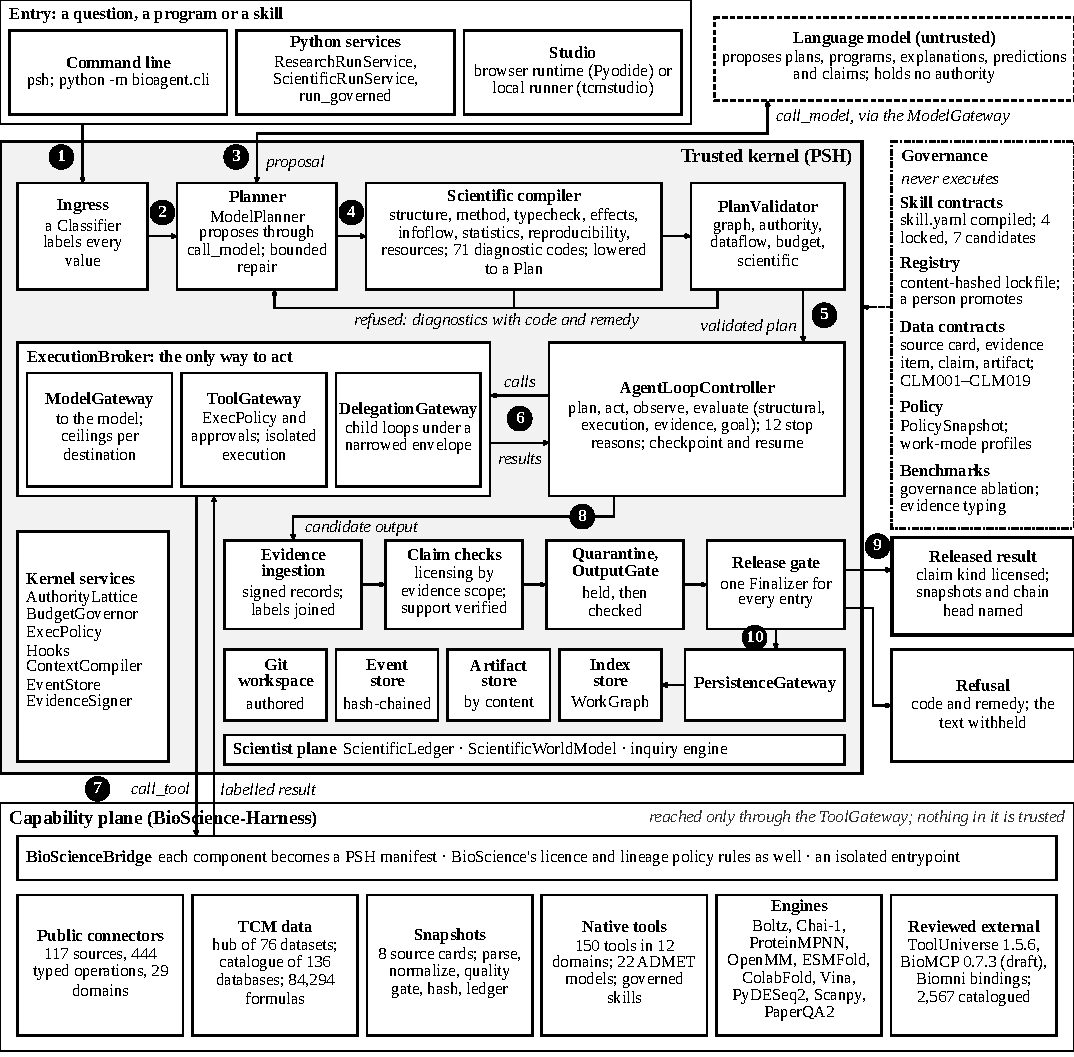
\includegraphics[width=\textwidth]{IEEE_Fig_Architecture.pdf}
\caption{The TCMScience agent architecture, with each component named as in the code.
(1)~A request enters through the command line, the Python services or Studio and is labelled
at ingress. (2)~It passes to the planner, which (3)~obtains a proposal from the language
model only through \texttt{call\_model} and the ModelGateway. (4)~The scientific compiler
checks the proposed program in eight passes (structure, method, typecheck, effects, infoflow,
statistics, reproducibility, resources; 71 diagnostic codes) and lowers it to a typed plan; a
refused program returns to the planner with each diagnostic's code and remedy, for a bounded
number of repairs. (5)~The PlanValidator checks the whole plan (graph, authority, dataflow,
budget, scientific) before any step runs. (6)~The AgentLoopController acts only through the
ExecutionBroker's three calls (model, tool, delegate) and stops for one of 12 named reasons.
(7)~Tool calls cross the BioScienceBridge into the capability plane and return as labelled
results. (8)~The loop's candidate output passes evidence ingestion and claim checks and is
held in quarantine and checked by the OutputGate; (9)~it leaves only through one release
gate, either as a result whose claim kind its evidence licenses or as a refusal with its code
and remedy. (10)~Validated state is committed through the PersistenceGateway to four stores,
and every gate's decision is appended to the hash-chained event store. Governance constrains
the kernel and never executes. Solid lines, execution; dashed, an untrusted component or a
constraint.}
\label{fig:architecture}
\end{figure*}

\begin{figure}[!t]
\centering
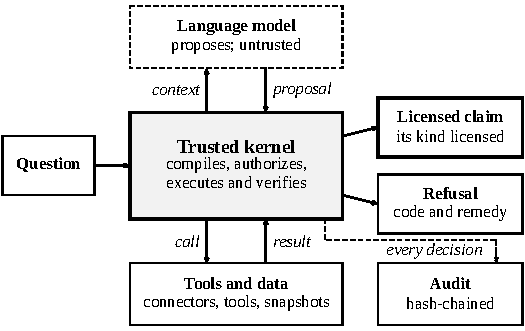
\includegraphics[width=\columnwidth]{IEEE_Fig_Minimal.pdf}
\caption{TCMScience in brief. The language model only proposes. The trusted kernel compiles,
authorizes, executes and verifies every step, calls the model and the tools itself, and
releases a claim only of a kind its evidence licenses; otherwise it refuses, with a code and
a remedy. Every decision is appended to a hash-chained audit. Dashed box, untrusted; dashed
arrow, a record.}
\label{fig:minimal}
\end{figure}
